\documentclass{article}

\usepackage{amsmath}

\usepackage{mathptmx}           
\usepackage{graphicx}           
\usepackage{url}            
\usepackage{subcaption}    


\usepackage[a4paper,margin=2cm]{geometry}

\usepackage{natbib} 
\usepackage[numbered, framed]{mcode}

\usepackage{lipsum}

\usepackage{epstopdf}
%\epstopdfsetup{outdir=./}

\begin{document}

\author{H. Blum, D. Cavezza, A. Paudice and M. Rohbeck\\
 Machine Learning CO395\\
  Imperial College London}
\date{\today}
\title{Assignment 3: Neural Networks}
\maketitle

\section{Validation}
In our second assignment, we apply neural networks to the emotion recognition problem. We use the Neural Network Toolbox provided by MATLAB to train and compare the performance of different neural networks on the dataset at our disposal, in order to find the best training algorithm along with the best parameter configuration.\\
We compare four different training algorithms:
\begin{itemize}
	\item Standard gradient descent backpropagation (\verb$traingd$ in MATLAB);
	\item Gradient descent with adaptive learning rate (\verb$traingda$);
	\item Gradient descent with momentum (\verb$traingdm$)
	\item Resilient backpropagation (\verb$trainrp$).
\end{itemize}
%In this section we describe our implementation of:
%\begin{itemize}
	%\item selection of the best set of parameters for each algorithm;
	%\item evaluation of NN's performance on unseen data.
%\end{itemize}

Our Neural Network has an input layer of size 45 (the number of features) and an output layer of 6 neurons (the number of classes). The network tries to approximate a 6-output function in which every output is 0 except for the $i$-th one, which is 1 if the sample is in class $i$. To convert the output of the neural network into a class value, we use the function \verb$NNout2labels$ that has been provided to us: it returns the index of the maximum output as the class value.

\subsection{Implementation}
In the first part, we use cross-validation to select the best performing algorithm on the dataset and the best parameter configuration for it. Cross-validation is performed by splitting the dataset into 10 folds and using 9 folds for training and 1 for validation; iteratively, each fold is in turn used for validation, and ultimately the algorithm and parameter set that yield the best average performance over the folds are chosen.\\
For each algorithm, we compare several network topologies and parameter values in all their combinations. The tested values are shown in Table~\ref{tab:parameters}.
\begin{table}
	\centering
	\caption{Parameters tested}
	\label{tab:parameters}

		\begin{tabular}{|l|l|l|}
		\hline
		Neurons per hidden layer & \multicolumn{2}{l|}{From 6 to 45} \\\hline
		Hidden layers		& \multicolumn{2}{l|}{[1, 2]} \\\hline
		\verb$traingd$	&	Learning rate		&	[5 3 1 0.5 0.3 0.1 0.05 0.03 0.01] \\\hline
		\verb$traingda$	&	Learning rate & [1 0.1 0.01] \\\cline{2-3}
										& LR decrease ratio	&	[0.7 0.07 0.03] \\\cline{2-3}
										& LR increase ratio & [1.4 2 5]	\\\hline
		\verb$traingdm$	&	Learning rate	&	[5 3 1 0.5 0.3 0.1 0.05 0.03 0.01]	\\\cline{2-3}
										&	Momentum			&	[0.9 0.95]	\\\hline
		\verb$trainrp$	&	Delta increase	&	[1.4 1.3 1.2 1.1]	\\\cline{2-3}
										&	Delta decrease	&	[0.7 0.5 0.3 0.07 0.05 0.03]	\\
		\hline		
		\end{tabular}
\end{table}
For further details on the criteria that led to those choices, see the answer to Question 1.\\
The trained network has the default architecture returned by the function \verb$feedforwardnet$: it uses sigmoid activation functions in the hidden layers and linear activation functions for the output neurons. As mentioned in Mitchell's book, with sigmoid functions in the hidden layer and linear outputs we can approximate arbitrary functions using two hidden layers and continuous functions using only one hidden layer.
Our choice for the performance measure falls onto the Mean Squared Error (MSE): this is the error function corresponding to the chosen output activation function.\\
A known problem of the basic training algorithm regards the random choice of the initial weights: a bad choice may lead the MSE to converge to a local minimum different from the global one. To soften the effect of the random choice, in each trial we train the network five times with the same parameters and take as a performance measure the minimum MSE on the validation set.\\
As a technique to avoid overfitting, we rely on the Early Stopping implemented by default in NNTools. This technique stops the training before the maximum number of iterations of gradient descent is performed: when the MSE on the validation set starts rising, the algorithm keeps executing for a maximum of \verb$net.trainParam.max_fail$ iterations; if the error does not decrease in these iterations, the algorithm stops and the weights of the network are set to the values that achieved the minimum error on the validation set, otherwise it continues.\\
\subsubsection*{Code}
For splitting the dataset into folds, we use the same function as in the previous coursework, which performs \emph{stratified} cross-validation: each fold contains approximately the same proportion of examples in every class as the whole dataset. It is implemented in the file \verb$getFoldsPartitioning.m$.\\
The files \verb$crossValidate.m$, \verb$validateNeuralNetwork.m$ and \verb$repeatNNTraining.m$ implement the cross-validation. The function \verb$crossValidate$ requires in input the algorithm to be validated and the dataset. The outputs are:
\begin{itemize}
	\item \verb$parameters$: a cell array containing all the parameter values tested in the cross-validation; each cell contains an array of values for a single parameter. For instance, in \emph{traingd} the first cell contains the tested values for the number of neurons per hidden layer, the second cell contains the numbers of hidden layers and the third one all the learning rates tested;
	\item \verb$mserrors$: a multidimensional array containing the average MSE computed over all the validation sets for each combination of parameters; the indices of each element in the array correspond to the indices of the parameter values in \verb$parameters$.
\end{itemize}
Since the cross-validation requires time to be completed, the function saves the performance computed on every validation fold by every parameter configuration as a precaution.
\begin{lstlisting}[breaklines=true]
function [ parameters, mserrors ] = crossValidate( algorithm, attributes, labels )

% Get the indices of the 10 folds as a cell array of 10 indices arrays
foldsIndices = getFoldsPartitioning(labels,10,true);

[parameters, numParams] = getParameters(algorithm);

mserrors = zeros(numParams);
for i=1:10
    disp(['Testing fold ' num2str(i)]);
    trainingSetIndices = getTrainingSetIndexed(foldsIndices,i);
    validationSetIndices = foldsIndices{i};
    
    mserrorsPerFold = validateNeuralNetwork(algorithm,parameters,attributes,labels,trainingSetIndices,validationSetIndices);
    save([algorithm '_msErrorsFold' num2str(i) '.mat'],'parameters','mserrorsPerFold');
    
    mserrors = mserrors+mserrorsPerFold;
end
% Average the accuracies
mserrors = mserrors./10;
save([algorithm '_avgmsErrors.mat'],'parameters','mserrors');


end


\end{lstlisting}
For each validation fold, the function \verb$validateNeuralNetwork$ is called. The main structure of this function has a \verb$switch$ statement, which checks the algorithm that is being tested; according to the algorithm, it loops over all the parameters that we need to test and calls the function \verb$repeatNNTraining$ for each parameter combination.
\begin{lstlisting}[breaklines=true]
function [ mserrors ] = validateNeuralNetwork( algorithm, parameters, attributes, labels, trainingSetIndices, validationSetIndices )
% attributes and labels must be in CBC format (rows representing single
% examples, columns attributes; one-column labels)

[attributesNN,labelsNN] = ANNdata(attributes,labels);

% Set common parameters
neuronsPerLayer = parameters{1};
hiddenLayers = parameters{2};

switch algorithm
    case 'traingd'
        % Define the candidate parameter values (learning rates)
        learningRates = parameters{3};
        mserrors = zeros(length(neuronsPerLayer), length(hiddenLayers), length(learningRates));
        
        for a = 1:length(neuronsPerLayer)
            npl = neuronsPerLayer(a);
            for b = 1:length(hiddenLayers);
                l = hiddenLayers(b);
                % Create a NN with l layers and npl neurons
                % per layer
                net = feedforwardnet(repmat(npl,1,l),algorithm);
                % To avoid showing the performance window
                net.trainParam.showWindow = 0;
                for c = 1:length(learningRates);
                    lr = learningRates(c);
                    % Set learning rate
                    net.trainParam.lr = lr;
                    
                    disp(['Testing parameters npl=' num2str(npl)...
                                ' l=' num2str(l) ' lr=' num2str(lr)]);

                    mserrors(a,b,c) = repeatNNTraining(net, ...
                                attributesNN, labelsNN, trainingSetIndices, ...
                                validationSetIndices);
                    
                end
                
            end
            
        end
\end{lstlisting}
The function \verb$repeatNNTraining$ first sets the training and validation sets for the training algorithm,
\begin{lstlisting}[firstnumber=17]
    net.divideFcn = 'divideind';
    net.divideParam.trainInd = trainingSetIndices;
    net.divideParam.valInd = validationSetIndices;
    net.divideParam.testInd = [];
\end{lstlisting}
then it configures the input and output layers' sizes and trains the network,
\begin{lstlisting}[firstnumber=22]
    % Set up input and output layer
    NN{j} = configure(net, attributesNN, labelsNN);
    % Train network
    [NN{j}, trainRecord] = train(NN{j}, attributesNN, labelsNN);
\end{lstlisting}
and finally keeps the performance value computed on the validation set for the following operations; this value can be retrieved via the field \verb$best_vperf$ of the struct \verb$trainRecord$.
\begin{lstlisting}[firstnumber=30]
    perfs(j) = trainRecord.best_vperf;
\end{lstlisting}
At the end of the five iterations, the network that performed best on the validation set is returned, along with the error measured.

\subsection{Selected parameters}
The parameters that reach the minimum average MSE over the 10 validation sets are:
\begin{itemize}
	\item \textbf{Algorithm:} Resilient backpropagation (\verb$trainrp$)
	\item \textbf{Neurons per layer:} 14
	\item \textbf{Layers:} 2
	\item \textbf{Delta increase:} 1.3
	\item \textbf{Delta decrease:} 0.5
\end{itemize}

\section{Performance evaluation}

\subsection{Implementation}
For evaluating the performance of the chosen model on unseen data, we use cross-validation with three sets:
\begin{itemize}
	\item a training set, used to execute gradient descent;
	\item a validation set, used to determine the termination condition and avoid overfitting, as well as optimizing the parameters;
	\item a test set, used for evaluating the performance.
\end{itemize}
The procedure is aimed at verifying the performance of the model obtained via cross-validation on data that have been used neither for training nor for parameter optimization.\\
The dataset is divided again in 10 folds. In each of the 10 iterations, one fold is used as test set, one as validation set and the remaining 8 as training set. The network is trained on the training set and the parameters are optimized on the validation set; in this phase the performance measure used, both for training and validation, is MSE as in the previous section. As before, we repeat the training 5 times and take the network that achieved the minimum error on the validation set. The resulting network is then tested on the test set in terms of confusion matrix and derived performance measures (accuracy, precision, recall). Since in each iteration the optimization is done on a different validation set, it may happen (and it actually does) that different parameter configurations are tested on different folds: in this way, we are truly estimating the performance of the entire approach we use to train and optimize the network, not just of a single trained network.\\

\subsubsection*{Code}
The implementation is provided in the file \verb$performanceEstimation.m$. The function first sets up the training, validation and test sets, and then loops over the training algorithms. For each algorithm, it calls \verb$validateNeuralNetwork$ (line 36) to obtain the MSE values for all the configuration parameters. The minimum MSE is recorded for each algorithm and finally the best MSE over all the algorithms on the given validation set is found.\\
\begin{lstlisting}[breaklines=true]
function [confusionMatrix, accuracy, precision, recall, f1] = performanceEstimation(attributes, labels)

algorithms = {'traingd', 'traingda', 'traingdm', 'trainrp'};
n_alg = length(algorithms);
confusionMatrix = zeros(6);
accuracyFolds = zeros(10,1);
precisionFolds = zeros(10,6);
recallFolds = zeros(10,6);
f1Folds = zeros(10,6);

% Get the indices of the 10 folds as a cell array of 10 indices arrays
foldIndices = getFoldsPartitioning(labels,10,true);

for i = 1:10 % iterate over 10 test folds
    % Split: Test- 1 Fold (i) Validation- 1 Fold (k) Training-8
    testSetIndices = foldIndices{i};
    k = mod(i,10)+1;
    validationSetIndices = foldIndices{k};
    trainingSetIndices = [];
    for j=1:10
        if j~=i && j~=k
            trainingSetIndices = [trainingSetIndices foldIndices{j}];
        end
    end
    
    % find optimal Parameters with training and validation set
    bestPerformingAlgorithm = 1;
    bestMSE = Inf;
    optimalParameters = [];
    
    for k = 1:n_alg
        parameters = getParameters(algorithms{k});
        
        disp(['Fold ' num2str(i) ' Algorithm: ' algorithms{k}]);
        
        mserrorsAlgorithm = validateNeuralNetwork(algorithms{k}, parameters, ...
            attributes, labels, trainingSetIndices, validationSetIndices);
        % idx is the index of the minimum in the linearized
        % mserrorsAlgorithm
        [minMSE, idx] = min(mserrorsAlgorithm(:));
        % Get the corresponding indices in the multidimensional array
        idxParameters = cell(1,length(parameters));
        [idxParameters{:}] = ind2sub(size(mserrorsAlgorithm), idx);
        
        if(minMSE<bestMSE)
            bestMSE = minMSE;
            bestPerformingAlgorithm = k;
            optimalParameters = zeros(length(parameters),1);
            for j=1:length(parameters)
                optimalParameters(j) = parameters{j}(idxParameters{j});
            end
        end
    end
    
    optimalAlgorithm = algorithms{bestPerformingAlgorithm};
\end{lstlisting}

The optimized network is used to perform a test on the test set and the corresponding confusion matrix is recorded. Both the optimal network and the confusion matrix are saved to the file \verb$confMatrixFold<i>.mat$ for subsequent use.
\begin{lstlisting}[firstnumber=57,breaklines=true]
    % Configure the best training algorithm with the optimal parameter
    % configuration
    net = configureNeuralNetwork(optimalAlgorithm,optimalParameters);
    % Train the network 5 times and get the best network
    [attributesNN,labelsNN] = ANNdata(attributes,labels);
    [~,net] = repeatNNTraining(net,attributesNN,labelsNN,trainingSetIndices,validationSetIndices);
    
    % Compute performance on test set
    predictions = NNout2labels(sim(net,attributesNN(:,testSetIndices)));
    confMatrixFold = getConfusionMatrix(labels(testSetIndices),predictions,6);
    save(['confMatrixFold' num2str(i)],'net','confMatrixFold');
    
    accuracyFolds(i) = sum(diag(confMatrixFold))/length(testSetIndices); % The sum of all the elements in confMatrixFold is
                                                                         % equal to the size of the test set
    precisionFolds(i,:) = diag(confMatrixFold)./sum(confMatrixFold,1)';
    recallFolds(i,:) = diag(confMatrixFold)./sum(confMatrixFold,2);
    for j=1:6
        if(precisionFolds(i,j)+recallFolds(i,j)==0)
            f1Folds(i,j)=0;
        else
            f1Folds(i, j) = 2* precisionFolds(i,j).*recallFolds(i,j) ...
                ./ (precisionFolds(i,j) + recallFolds(i,j));
        end
    end
    confusionMatrix = confusionMatrix+confMatrixFold;
end
    
accuracy = mean(accuracyFolds);
precision = mean(precisionFolds,1);
recall = mean(recallFolds,1);
f1 = mean(f1Folds,1); 
            
end
\end{lstlisting}
To compute the total confusion matrix, we sum the confusion matrices of the folds. To compute the performance statistics of the whole network, we average the performance statistics over the folds.\\
For computing the performance on noisy data, we use again cross-validation with training, validation and test sets, but this time we skip the phase of parameter optimization. For testing on each fold we use the 10 optimal networks found on the clean data and saved in the respective \verb$.mat$ files. We train such networks on the training set and perform early stopping by computing the error on the validation set; finally, we get the confusion matrix of the trained network on the test fold.

\subsection{Performance results}
The performance results of the network trained and tested on clean data are shown in Figure~\ref{fig:perfClean}. The accuracy is higher than the one recorded for decision trees (79.8\% against 74.7\%). As in decision trees, also here the classes \emph{anger} and \emph{sadness} have the worst performance figures. It is possible that the Action Units used as features are not sufficiently able to discriminate these emotions from the other ones; therefore:
\begin{itemize}
	\item we have low precision since many sample points belonging to the other classes are confused with \emph{anger} or \emph{sadness};
	\item we have low recall since many \emph{anger} and \emph{sadness} sample points are not correctly recognized by the network.
\end{itemize}
The emotions with the best performance are \emph{happiness} and \emph{surprise}: they exhibit an F-measure of 91.6\% and 89.4\% respectively. Probably, this is because there are AUs whose activation is a strong indication of those emotions: for instance, \emph{happiness} is highly related to the activation of AU12, which corresponds to smile; \emph{surprise}, instead, is strongly related to the activation of AU2, AU1 (Outer and Inner Brow Raiser), AU27 (Mouth Stretch) and AU26 (Jaw Drop)\footnote{\url{https://en.wikipedia.org/wiki/Facial_Action_Coding_System}}. These were the AUs at the higher levels of the corresponding decision trees in the previous exercise: these features are likely to be as discriminative in neural networks.\\
Similar observations can be done for noisy data, as shown in Figure~\ref{fig:perfNoisy}. There is a general reduction in terms of performance, particularly for the recall of \emph{anger}, which dramatically decreases to 6.9\%. However, for the other classes the performance remains at high values, over 80\% of $F_1$ for \emph{happiness} and \emph{surprise}.
\begin{figure}
    \center
    \subcaptionbox{Confusion matrix}{
        $\begin{bmatrix}
					True\backslash Predicted & anger & disgust & fear & happiness & sadness & surprise \\ 
					anger & 83 & 12 & 9 & 4 & 23 & 1 \\
					disgust & 14 & 158 & 3 & 5 & 15 & 3 \\
					fear & 0 & 2 & 85 & 3 & 10 & 19 \\
					happiness & 0 & 4 & 5 & 201 & 6 & 0 \\
					sadness & 11 & 18 & 7 & 7 & 86 & 3 \\
					surprise & 1 & 0 & 10 & 3 & 5 & 188 \\
				\end{bmatrix}$
    }
		\\\center
    \subcaptionbox{Performance metrics}{
        \begin{tabular}{c | c c c | c}
Class & Precision & Recall & $F_1$ & Accuracy \\
\hline\hline
anger & 69.8\% & 63.0\% & 65.5\% &\\ 
disgust & 81.6\% & 79.8\% & 80.3\% &\\ 
fear & 72.4\% & 71.4\% & 70.8\% &	79.8\%\\ 
happiness & 90.6\% & 93.1\% & 91.6\% &\\ 
sadness & 60.8\% & 65.1\% & 62.3\% &\\ 
surprise & 88.4\% & 90.9\% & 89.4\% &\\ 
        \end{tabular}
    }%
    
    \caption{Performance of Neural Network on clean data}
		\label{fig:perfClean}
\end{figure}

\begin{figure}
    \center
    \subcaptionbox{Confusion matrix}{
        $\begin{bmatrix}
					True\backslash Predicted & anger & disgust & fear & happiness & sadness & surprise \\ 
					anger & 6 & 16 & 21 & 9 & 32 & 4 \\
					disgust & 2 & 151 & 12 & 7 & 12 & 3 \\
					fear & 1 & 13 & 133 & 11 & 14 & 15 \\
					happiness & 3 & 8 & 14 & 173 & 6 & 5 \\
					sadness & 2 & 14 & 16 & 5 & 61 & 12 \\
					surprise & 1 & 4 & 18 & 7 & 10 & 180 \\
				\end{bmatrix}$
    }
		\\\center
    \subcaptionbox{Performance metrics}{
        \begin{tabular}{c | c c c | c}
Class & Precision & Recall & $F_1$ & Accuracy \\
\hline\hline
anger & 27.5\% & 6.9\% & 10.2\% &\\ 
disgust & 74.6\% & 80.7\% & 77.0\% &\\ 
fear & 62.5\% & 71.2\% & 66.5\% &	70.4\%\\ 
happiness & 81.9\% & 82.8\% & 81.8\% &\\ 
sadness & 45.6\% & 55.5\% & 49.6\% &\\ 
surprise & 82.3\% & 81.8\% & 81.9\% &\\ 
        \end{tabular}
    }%
    
    \caption{Performance of Neural Network on noisy data}
		\label{fig:perfNoisy}
\end{figure}

\section{Questions}
\subsection{Part A: Questions}
\subsubsection*{Question 1}
We chose the optimal topology and parameters through cross-validation. In detail, in each iteration we tested the performance of the chosen topology on the fold used as validation set. In the end, we averaged over the folds the performances of each topology and parameters configuration and chose the setting that showed the best average performance.\\
In the following our reasons behind the set of tested parameters:
\begin{itemize}
\item \textbf{Number of Layers:} We tested topologies with one and two hidden layers. Topologies with one hidden layer (two layers) can fit any bounded continuous function, while two-hidden-layer topologies can approximate arbitrarily well any real-valued function.
\item \textbf{Number of Neurons:} For each layer, a common practice is to use a number of neurons between the sizes of the input and the output layer. Choosing less neurons than the output leads to a data compression that may cause information loss before reaching the output and consequently underfitting. On the other hand, using too many neurons can easily lead to overfitting.
\end{itemize}
For the algorithms' parameters, we had to trade off the number of tests executed and the total time for testing. We chose parameters that covered different orders of magnitude where possible.
\begin{itemize}
\item \textbf{Learning Rate:} If the learning rate is too large, the gradient descent may diverge; conversely, if it is too small, the algorithm may require too many iterations to converge to the minimum error. Typical values are $0.1$ and $0.01$. Because this is an essential parameter, we tested three different values at three different orders of magnitude. The only exception was for the \verb$traingda$ algorithm: since it has 3 parameters to optimize, we had to reduce the number of learning rates tested.
\item \textbf{LR Decrease Ratio:} Typical values are $0.5$ and $0.7$, however we dropped 0.5 since we expect similar performance to the case of 0.7. On the other hand, we extended the range to a smaller order of magnitude to verify whether the usual value is suitable for our case or a very different value is needed. 
\item \textbf{LR Increase Ratio:} For this choice we followed similar criteria as the previous parameter. We started with the default value set by MATLAB, 1.4, and then tested significantly different values.
\item \textbf{Momentum:} We tested both values given as typical in the lecture slides.
\item \textbf{Delta Increase:} As a typical value, $1.2$ is given in the lecture slides. As this value has to be bigger than 1, we tested values around 1.2. We didn't consider higher orders of magnitude, as this would just lead to exploding update values and therefore most probably to a lot of oscillation and long converging times. In the end, our optimal parameter was close by the given value.
\item \textbf{Delta Decrease:} As a typical value, $0.5$ is given in the lecture slides. Again, we tested different values around this number and this time also tested values of smaller magnitude. Bigger magnitues were not possible as the parameter has to be smaller than 1. Our optimal parameter actually was $0.5$.
\end{itemize}
The optimal parameters for the different learning techniques are the following.
\begin{itemize}
\item \textbf{standard gradient descent:} \\ Neurons per layer = 18, Number of layers = 2, Learning rate (LR) = 0.5, Avg. Error = 0.0458
\item \textbf{adaptive gradient descent:}\\ Neurons per layer = 15, Number of layers = 2, Learning rate = 0.1, LR decrease rate = 0.7, LR increase rate = 1.4, Avg. Error = 0.0449
\item \textbf{gradient descent with momentum:}\\ Neurons per layer = 42, Number of layers = 1, Learning rate = 1, Momentum coefficient = 0.9, Avg. Error = 0.0679
\item \textbf{resilient backpropagation:}\\ Neurons per layer = 14, Number of layers = 2, Delta increase = 1.3, Delta decrease = 0.5, Avg. Error = 0.0444
\end{itemize}

\subsubsection*{Question 2}
\begin{figure}
 \centering
 \begin{subfigure}[b]{.8\textwidth}
   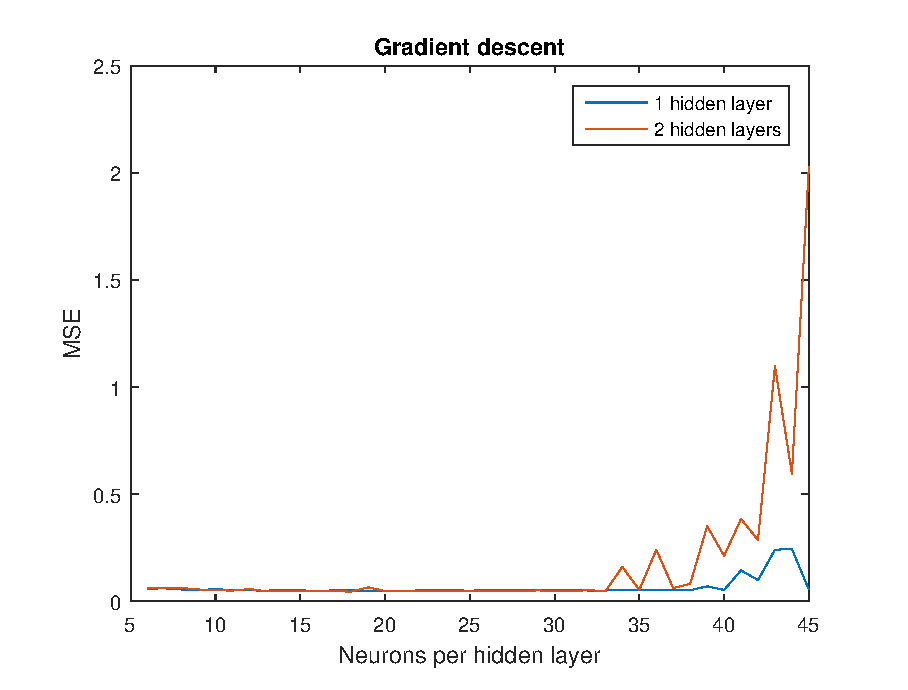
\includegraphics[width=\textwidth]{traingd_plot.eps}
 \end{subfigure}
 \begin{subfigure}[b]{.8\textwidth}
   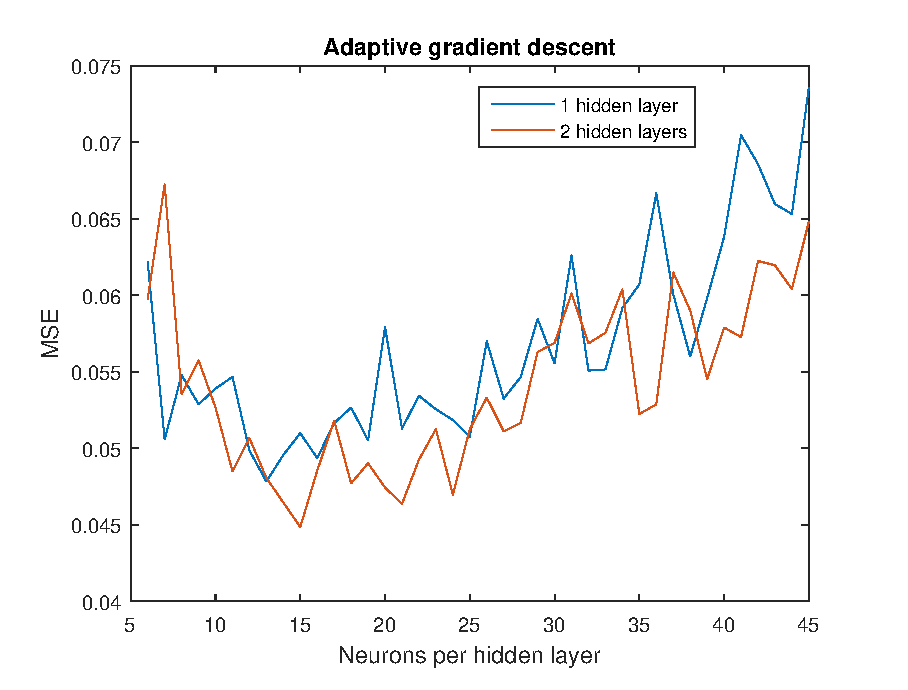
\includegraphics[width=\textwidth]{traingda_plot.eps}
 \end{subfigure}
\end{figure}
\begin{figure}
\ContinuedFloat
\centering
 \begin{subfigure}[b]{.8\textwidth}
   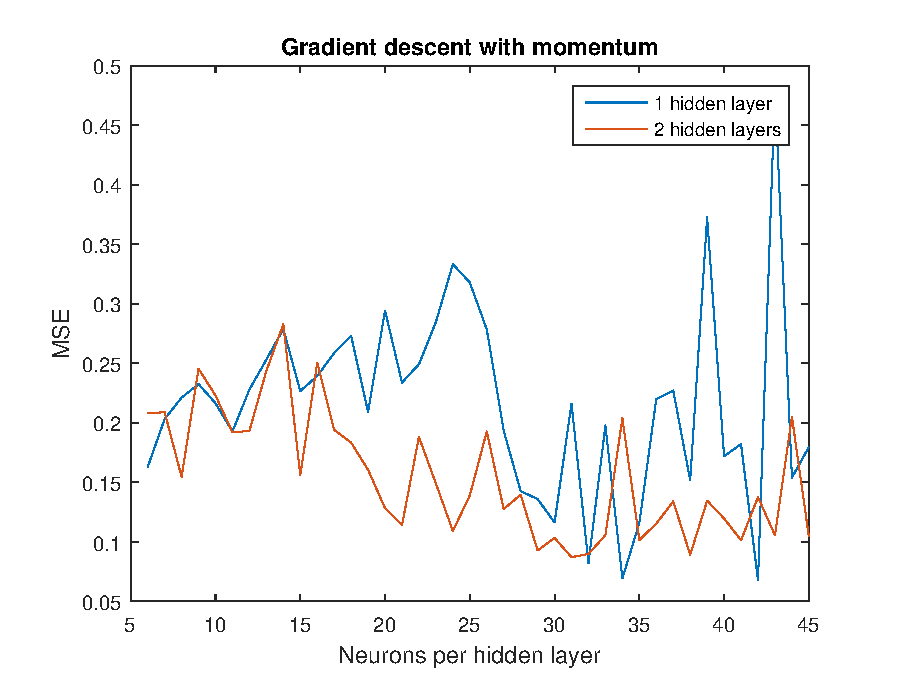
\includegraphics[width=\textwidth]{traingdm_plot.eps}
 \end{subfigure}
 \begin{subfigure}[b]{.8\textwidth}
   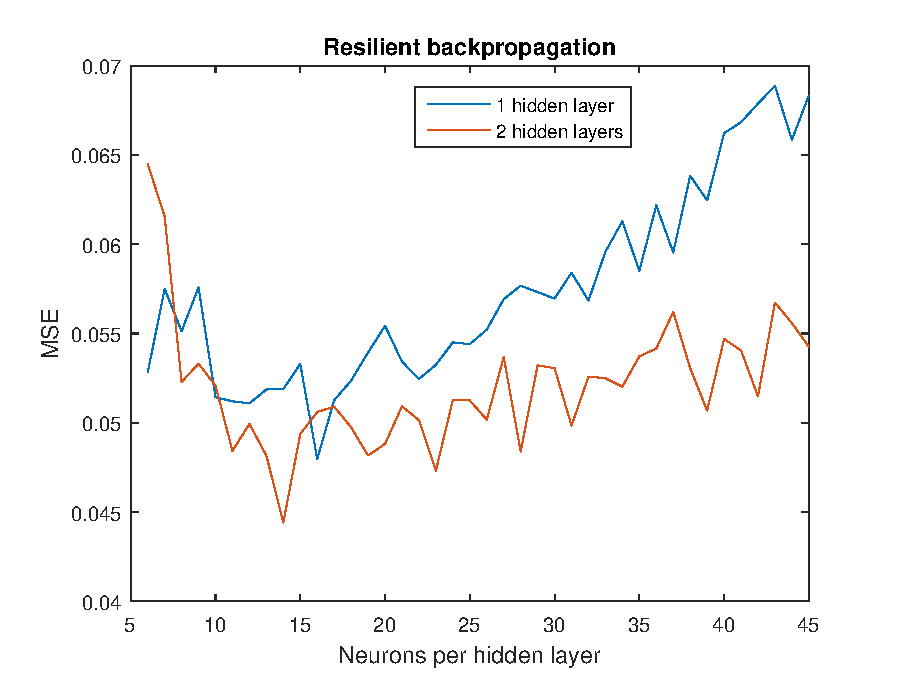
\includegraphics[width=\textwidth]{trainrp_plot.eps}
 \end{subfigure}
 \caption{Topology-Performance plots per algorithm}
 \label{fig:topologyPerformance}
\end{figure}
The plots in Figure~\ref{fig:topologyPerformance} represent the average MSE obtained on the 10 validation sets in cross-validation for all the different topologies tested. All the algorithm parameters are fixed to their optimal value found in cross-validation for each algorithm (reported in Question 1).

With the exception of the Momentum-Algorithm, the plots show increasing error for very large number of neurons in the hidden layer(s). In all plots the error becomes also bigger for very small numbers of hidden layer neurons. Our explanation is as follows.

In general, the number of neurons in the hidden layers defines the degrees of freedom in the approximation of the classification function. Therefore, very few hidden neurons lead to very few degrees of freedom, which would explain higher classification errors as the ANN may not be able to fit the training and validation data to a suitable degree (underfitting). On the other hand, a high degree of freedom increases the possibilities for overfitting, which again will cause a higher classification error on the validation set.

Especially interesting is the performance in relation to the number of hidden layers. This is linked to the size of the searched hypothesis space as 2-layer-ANNs can only approximate continuous functions whereas 3-layer-ANNs can approximate every function. This can now have 2 contrary effects. On one hand, with a bigger hypothesis space the ANN might be able to find a better fitting hypothesis and therefore perform better. On the other hand, this is linked to a greater possibility of overfitting, as it is much more difficult to find the best hypothesis given the limited data we have. Both aspects are shown in the plots. For the standard gradient descent, the network with 1 hidden layer becomes increasingly bad for large numbers of neurons, but not nearly as bad as for a 2-layer-network, where there is a much higher possibility of overfitting. In contrast, we can see that the resilient backpropagation performs in general better with 2 layers than with 1. It is also the overall best performing algorithm and therefore it may be better able to handle a large hypothesis space.


\subsubsection*{Question 3}
Matlab already implemented \emph{early stopping} by default. Therefore the available data is divided into three subsets: the training, validation and test set (possibly empty). The first one is used to find the weights for the network. If the error on the validation set starts to increase for several iterations, which is an indication for overfitting, the process stops and the the weights which produce the minimum error on the validation set are returned.\\
Early stopping is not a 100\% safe method as it is possible that the error on the validation set will decrease again after an unknown number of steps, but as it also reduces the training time and therefore comes somehow with negative cost, it is especially a good first approach for our (limited) computing power.\\
\\
Another possible approach would be \emph{regularisation}. Regularisation is a mechanism to reduce the occurence of large weights. As large weights imply that some particular paths through the network are much more important than others, it could be more likely for overfitting to occur. Therefore, a penalization term depending on the input weights of the neurons is added to the original error function that is minimized in the training. For example, in L2-Regularisation the squares of the weights are added together:
\begin{align*}
    E_{new} = E_{original} + \lambda \sum \limits_{all\ weights} w^2
\end{align*}
$\lambda$ is a parameter that sets the balance between the original minimization of the error and the minimization of the weights-function. Therefore, regularization would include another parameter to optimise and therefore a multiplication of the computing time. Because the optimisation of our other parameters already took approximately two days, we had strong time constraints. \\
\\
Theoretically also other techniques, for example \emph{dropout}, are possible.\\
In the dropout-method, random network nodes are dropped out in every training iteration with a constant probability for each node. Therefore, the network architecture is randomized and every architecture is just trained for a small random subset of the training data. This intuitively reduces the chance that the network is overfitted to the training data set as actually the network with $n$ nodes represents an average of all the before trained dropout-architectures (out of the set of $2^n$ possible networks), where each network node is only trained with parts of the training data. On the other hand, with small amounts of training data, the dropout-technique can actually reduce the classification performance. In particular, the paper from Srivastava et al. referenced in the lecture slides shows that dropouts only reduce the classification error for MNIST classification training data sets of size 5000 or bigger, while for 100 training examples the classification error was bigger than without dropout. Therefore, we are not confident that the dropout-technique would improve our performance whereas the implementation effort would be big.\\
\\
Finally, one could also consider \emph{Data Augmentation} by using the noisy dataset additionally to the clean dataset.

\subsubsection*{Question 4}
\textbf{Disadvantages} \\
First of all using 6 different ANNs leads to a necessary implementation of a decision function, which classifies on the basis of the outputs of the six networks. As in the assignment before, there is no obvious best solution for this problem and therefore the choice of decision function is another parameter to optimize.\\
The task for each of the six networks is to find a boolean classifying function. If we assume that we test the networks with the same topologies as the first big network, each network can represent \textit{exactly} one boolean function as long as it has at least two layers. This leads to a huge risk of overfitting compared to the one network which only \textit{approximates} an arbitrary function and is therefore more robust to noise. Furthermore, as the parameters are optimised differently for each output class, each network is more specifically fit to the training data and this might be another risk of overfitting.\\
Moreover, training six networks requires more resources than training one slightly (only the output layer size differs) bigger network. In general, this corresponds to a significantly longer training time. Of course, the time consumption can be reduced by parallelizing the process of cross-validation because the networks are independent (see advantages).\\
\\
\textbf{Advantages} \\
As the networks are trained more specifically to recognize one class, this approach could lead to a better performance.\\
Because the output layer is smaller than for one big network, there are less weights to optimize in each network for the same topology. As a result, parallel cross-validation of six networks will be faster than the cross-validation of one big network, as long as one has the required computing power.\\
\\
As a conclusion, computing power is a relevant aspect for us and therefore we prefer one classification network.\\\\
\textbf{Combination of Outputs} \\
The combination of the output of the six networks is exactly the same problem which was solved in our last assignment. These could be reused, possibly with small modifications: 
\begin{itemize}
    \item \textbf{random choice:} This is still possible by using a threshold value. Every output with a bigger value than the threshold is considered for the random pick.
    \item \textbf{score-based decision:} Naturally, the output of the networks is also a score, i.e. this algorithm can be used without any modifications.
    \item \textbf{depth-based decision:} The depth of a tree is a specific property of a decision tree and therefore it is not easy to find a similar and meaningful property for neural networks. Of course you could use the number of layers, but as this varies just between two values, the algorithm would probably not perform well as there would be a lot of ties.
    \item \textbf{error-based decision:} As the error of the networks can be calculated just as the errors of the trees, this strategy is also possible to use without modification.
\end{itemize}


\subsection{Part B: Questions}
\subsubsection*{Question 1}
After performing a t-test, feedforward neural networks showed to have a significantly smaller classification error than our decision tree implementation on clean data. %TODO on clean or noisy data or both?
However, although for our specific test performance sample neural networks did better than decision tree, it is not possible to state general conclusions about the relative performance of these two models. 

First, it should be observed that a t-test just refers to a specific sample of test performance. This implies that the resulting difference between the two algorithms is just an estimate of the true difference. Thus, any conclusion beyond the sampled population is not guaranteed to be true. Second, in our case we compared the classification error of the algorithms and in general it could be possible that for other performance metrics the resulting t-test would be different. 

To summarize, it is not possible to say whether a specific learning algorithm is better than another based on the performance for a given problem. Rather, when analyzing the performance of the algorithms one should always consider the specific problem domain, the relevant performance metric and the available dataset.

\subsubsection*{Question 2}
We trained and tested decision trees and neural networks on the same training and test sets which leads to dependent samples. Because of this, we adopted a paired t-test. %TODO more explanation

\subsubsection*{Question 3}
Considering the classification error rather than the F1 measure has the advantage to avoid the so called multiple hypothesis comparison problem. Indeed adopting the F1 measure for this multi-class classification problem leads to 6 different measurements per test set, i.e one per emotion. As a result, the sample for the t-test consists of 10 six-element vectors. To compare the two algorithms in this way we have to apply 6 different t-tests (one per  emotion), which leads to the multiple hypothesis comparison problem. Testing simultaneously 6 hypothesis with a significance (i.e a probability of rejecting the null hypothesis when it is actually true) $\alpha=0.05$ leads to an overall error probability of $0.3$ which makes the test much less effective. 

\subsubsection*{Question 4}
Let's first analyze the case of reducing the number of folds. Reducing the number of folds leads to a smaller sample on which to perform the t-test. Then, the $SE$ term of the t-statistic increases and the resulting t value gets smaller. Moreover, as the degrees of freedom (df) are directly proportional to the sample size, the corresponding threshold will be bigger. As a result, having a smaller statistic to test against a higher threshold, the number of false rejections for the null hypothesis increases. 

Conversely, increasing the number of folds leads to a bigger t-statistic and a smaller threshold which in turn might lead us to accept the null hypothesis when it is actually false. In any case, it should be observed that increasing the number of folds, one should be aware to get folds with at least 30 examples. Indeed, 30 examples is the minimum sample size to approximate the individual differences between the two algorithm as realization of a normal random variable; this provides the theoretical ground for the validity of t-test.

Anyway, it is important to specify that there is no argument to believe that 10 folds represent the optimum for this specific test.

\subsubsection*{Question 5}
In the case of the decision trees learning, adding new emotions requires to grow additional decision trees (in particular as many decision trees as emotions added). It should be observed that retraining is required since adding new emotions to the dataset enriches the set of negative examples of the pre-existing classes. On the other hand, in the case of neural networks it is required to add as many additional output layers as new emotions, to retrain the network and to optimize it again with cross-validation.

%\bibliographystyle{plainnat}
%\bibliography{example}

\end{document}
